\usepackage[english]{babel}
\usepackage[T1]{fontenc}
\usepackage[utf8]{inputenc}
\usepackage{graphicx}
\usepackage{listings}
\usepackage{amsmath}
\usepackage{amssymb}
%\usepackage{amsthm}
\usepackage{ae,aecompl}
\usepackage{fix-cm}

\usetheme{Goettingen}
%\usetheme{Singapore}

\beamertemplatenavigationsymbolsempty

\title{On isotoxal tilings in plane and in space}
\author{Boróczki, Lajos - Molnár, Emil}
\date{CGTA Vorau 21.06.2011}

\begin{document}

\begin{frame}
  \maketitle
\end{frame}

\begin{frame}
  \mode<presentation>{\frametitle{Outline}}
  \tableofcontents
\end{frame}
\newpage

\section{Abstract}
\begin{frame}
  \tiny
Conference on Geometry - Theory and Applications\\
CGTA 2011, Vorau/Austria, June 20-24, 2011
\vfill
\normalsize
\begin{center} On isotoxal tilings in plane and in space\end{center}

\vfill
\tiny
\textbf{BORÓCZKI, Lajos} and \textbf{MOLNÁR, Emil}\\
Budapest University of Technology and Economics, MI Department of Geometry\\
E-mail: boroczki.lajos@gmail.com, emolnar@math.bme.hu\\
\vfill

http://www.math.bme.hu/~geometry
\vfill

\tiny
\textbf{Abstract.} The squared papers in our booklets, or the squared (maybe black and white)
pavements in the streets arise an amusing problem, first in the Euclidean plane:
How to deform the side segments of the square pattern, so that the side lines
further remain equal (congruent) to each other? More precisely, we require that
each congruent mapping of the new pattern, mapping any deformed side segment
onto another one, leaves the whole (infinitely extended) pattern of the plane
invariant (unchanged).
\vfill

It turns out, that there are exactly 14 types of such  edge  transitive
(isotoxal) quadrangle tilings, sometimes  with  two  different  forms  (e.g.
black and white) of quadrangles. Such a collection of tilings seems  to  be
very nice, perhaps also useful  for  decorative  pavements  in  streets, in flats, etc.
\vfill

We shall sketch the solution of the problem, that leads to  fine  (and
important)  mathematical  concepts  as  barycentric   triangulation   of   a
polygonal  tiling,  adjacency  (neighbour)  operations,  adjacency   matrix,
symmetry group of a tiling, D-symbols, first in  the  Euclidean  plane  ($E^2$)
then in the spherical ($S^2$) and hyperbolic ($H^2$)  planes  as  well  (sometimes
with infinite series). Moreover, the method can be extended by  computer  to
the homogeneous spaces to polyhedral tilings (in Thurston geometries).
\vfill

All these  in  $E^2$  can  be  discussed  in  an  enjoyable  way,  by  the
attractive computer program of our colleague István Prok  on  the  Euclidean
plane crystallographic  groups  with  a  nice  interactive  play  (for  free
download).
\vfill

The problem in the non-Euclidean planes (E. Molnár with  Z.  Lu\u{c}i\'{c}  and
M. Stojanovi\'{c} (1994)) and in the space $E^3$ (E. Molnár with A.W.M.  Dress  and
D.H. Huson (1993)) is more difficult.
\vfill

The doctor work of the first author extends the problem onto non-Euclidean
spaces as well by computer through the D-symbol machinery in a more complex
way.
\vfill

\end{frame}

\begin{frame}
  \center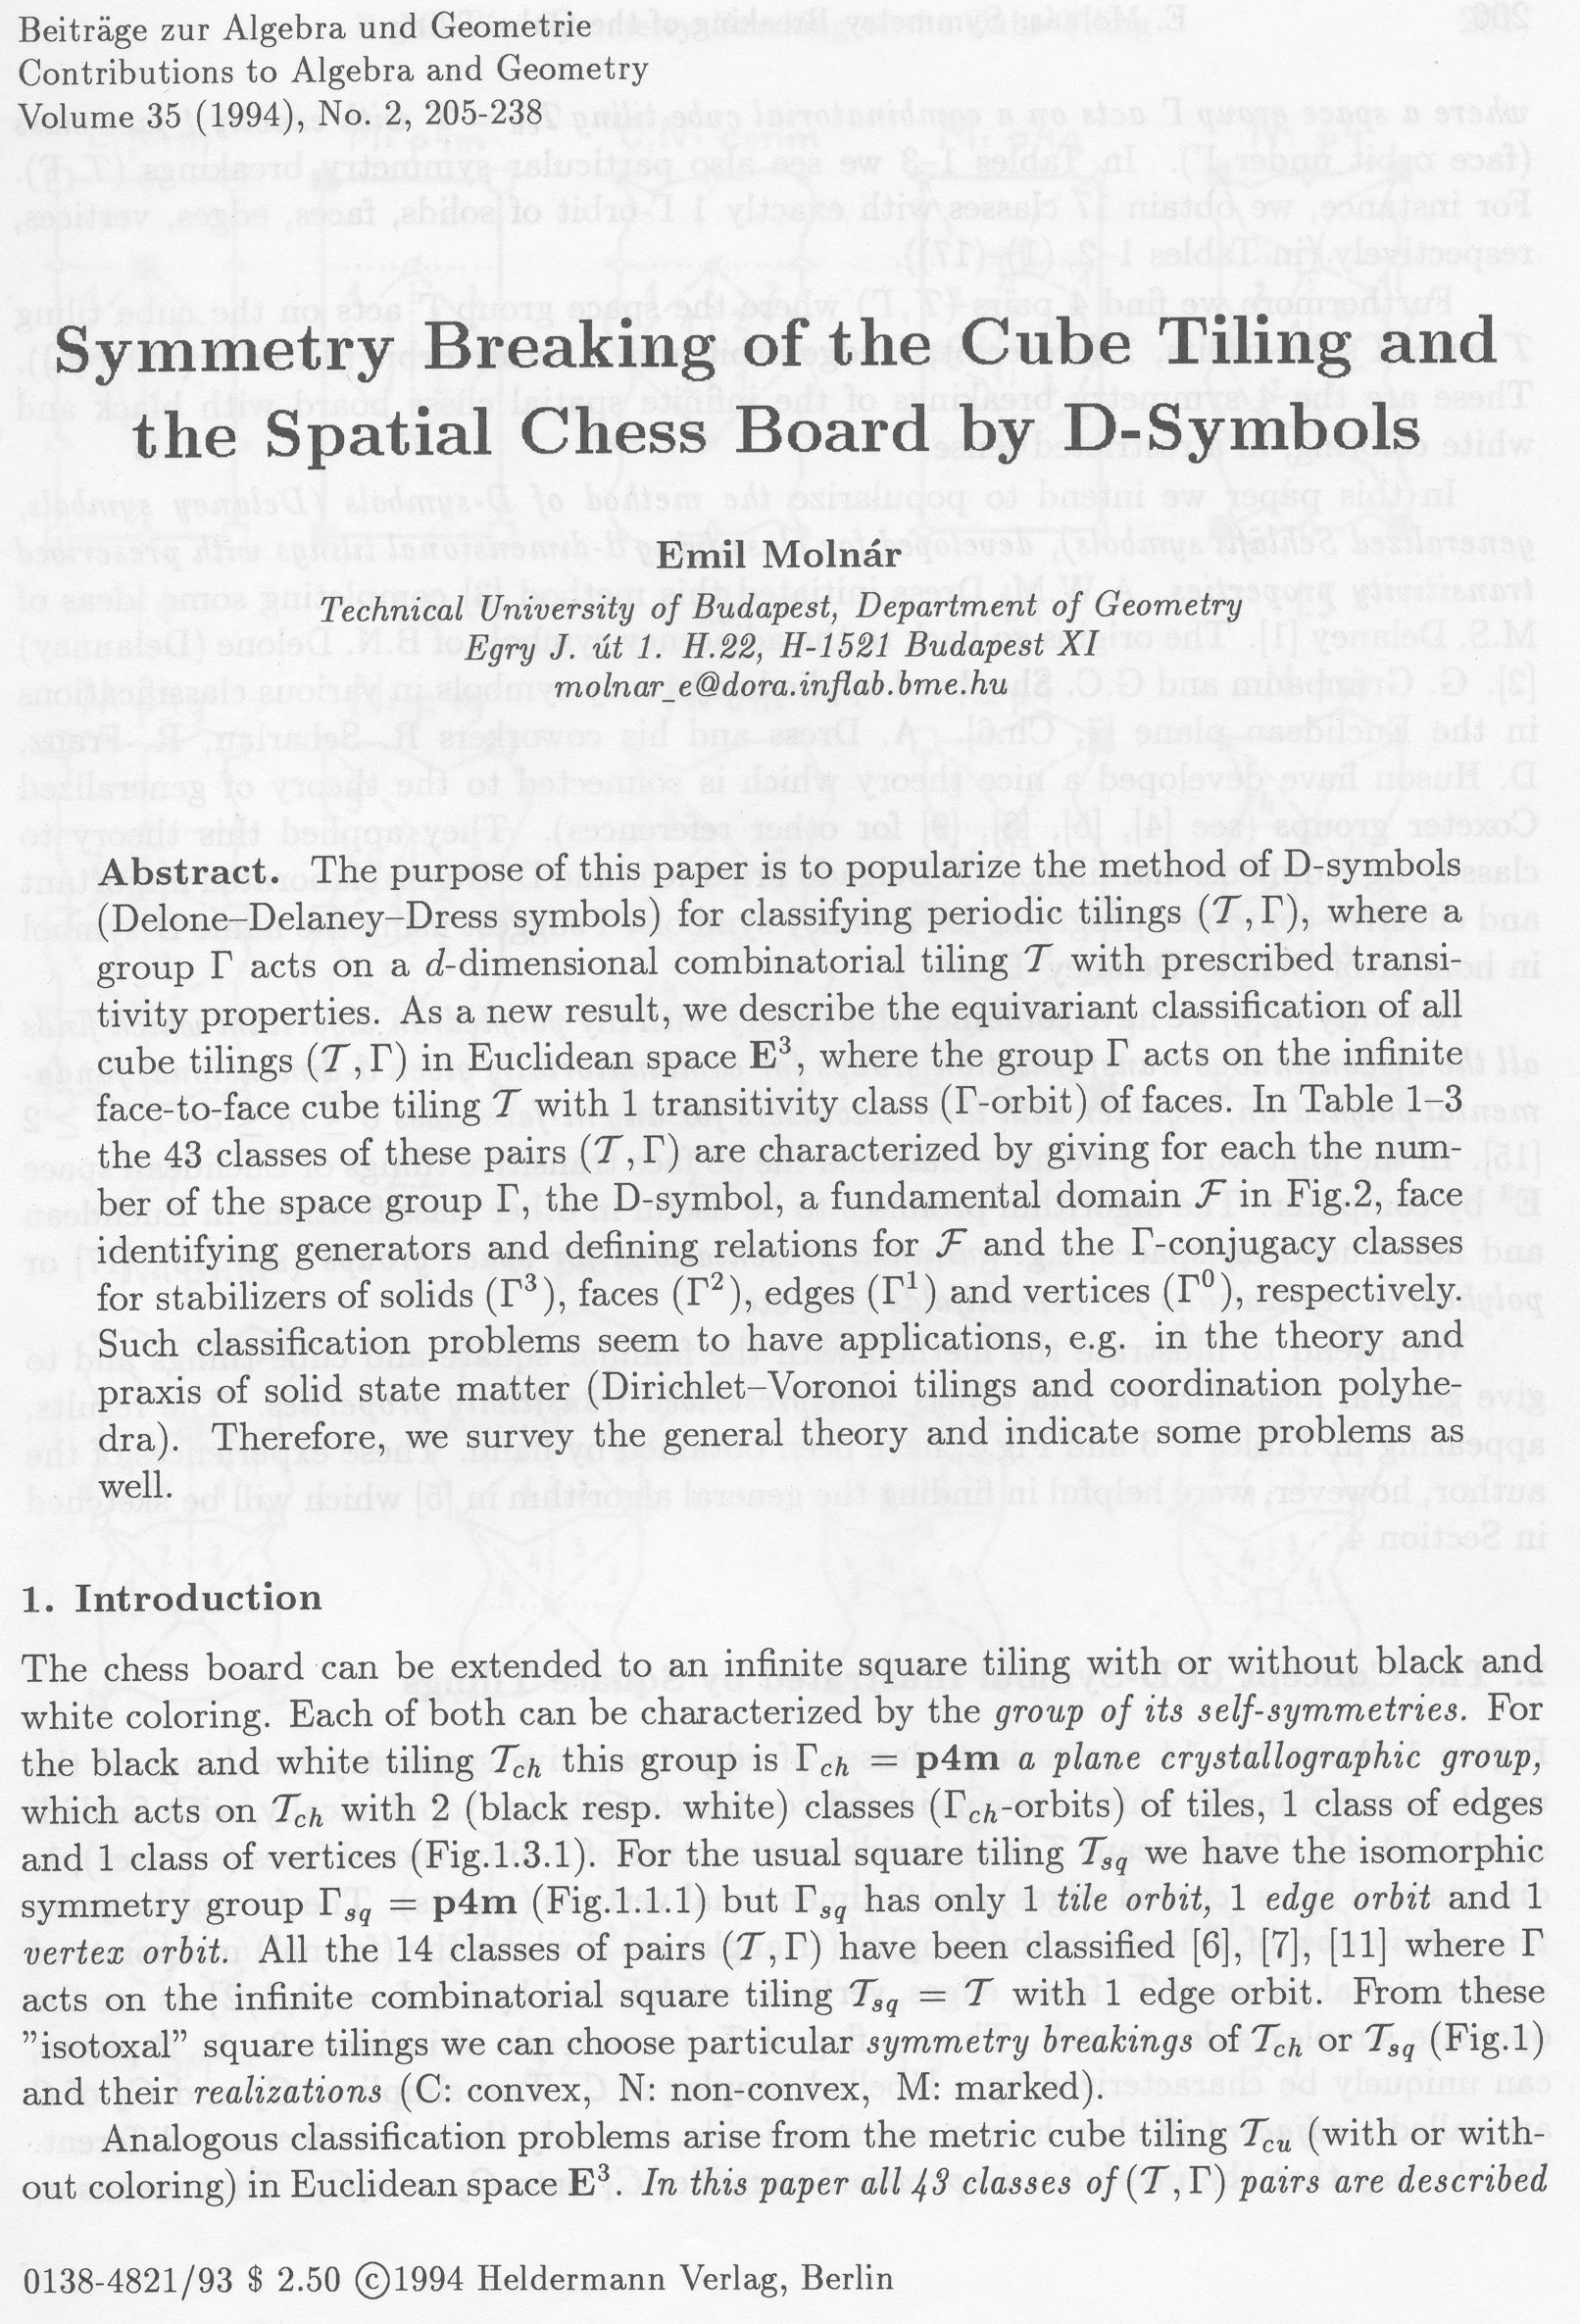
\includegraphics[width=0.6\textwidth]{illustration1.png}
\end{frame}

\begin{frame}
  \center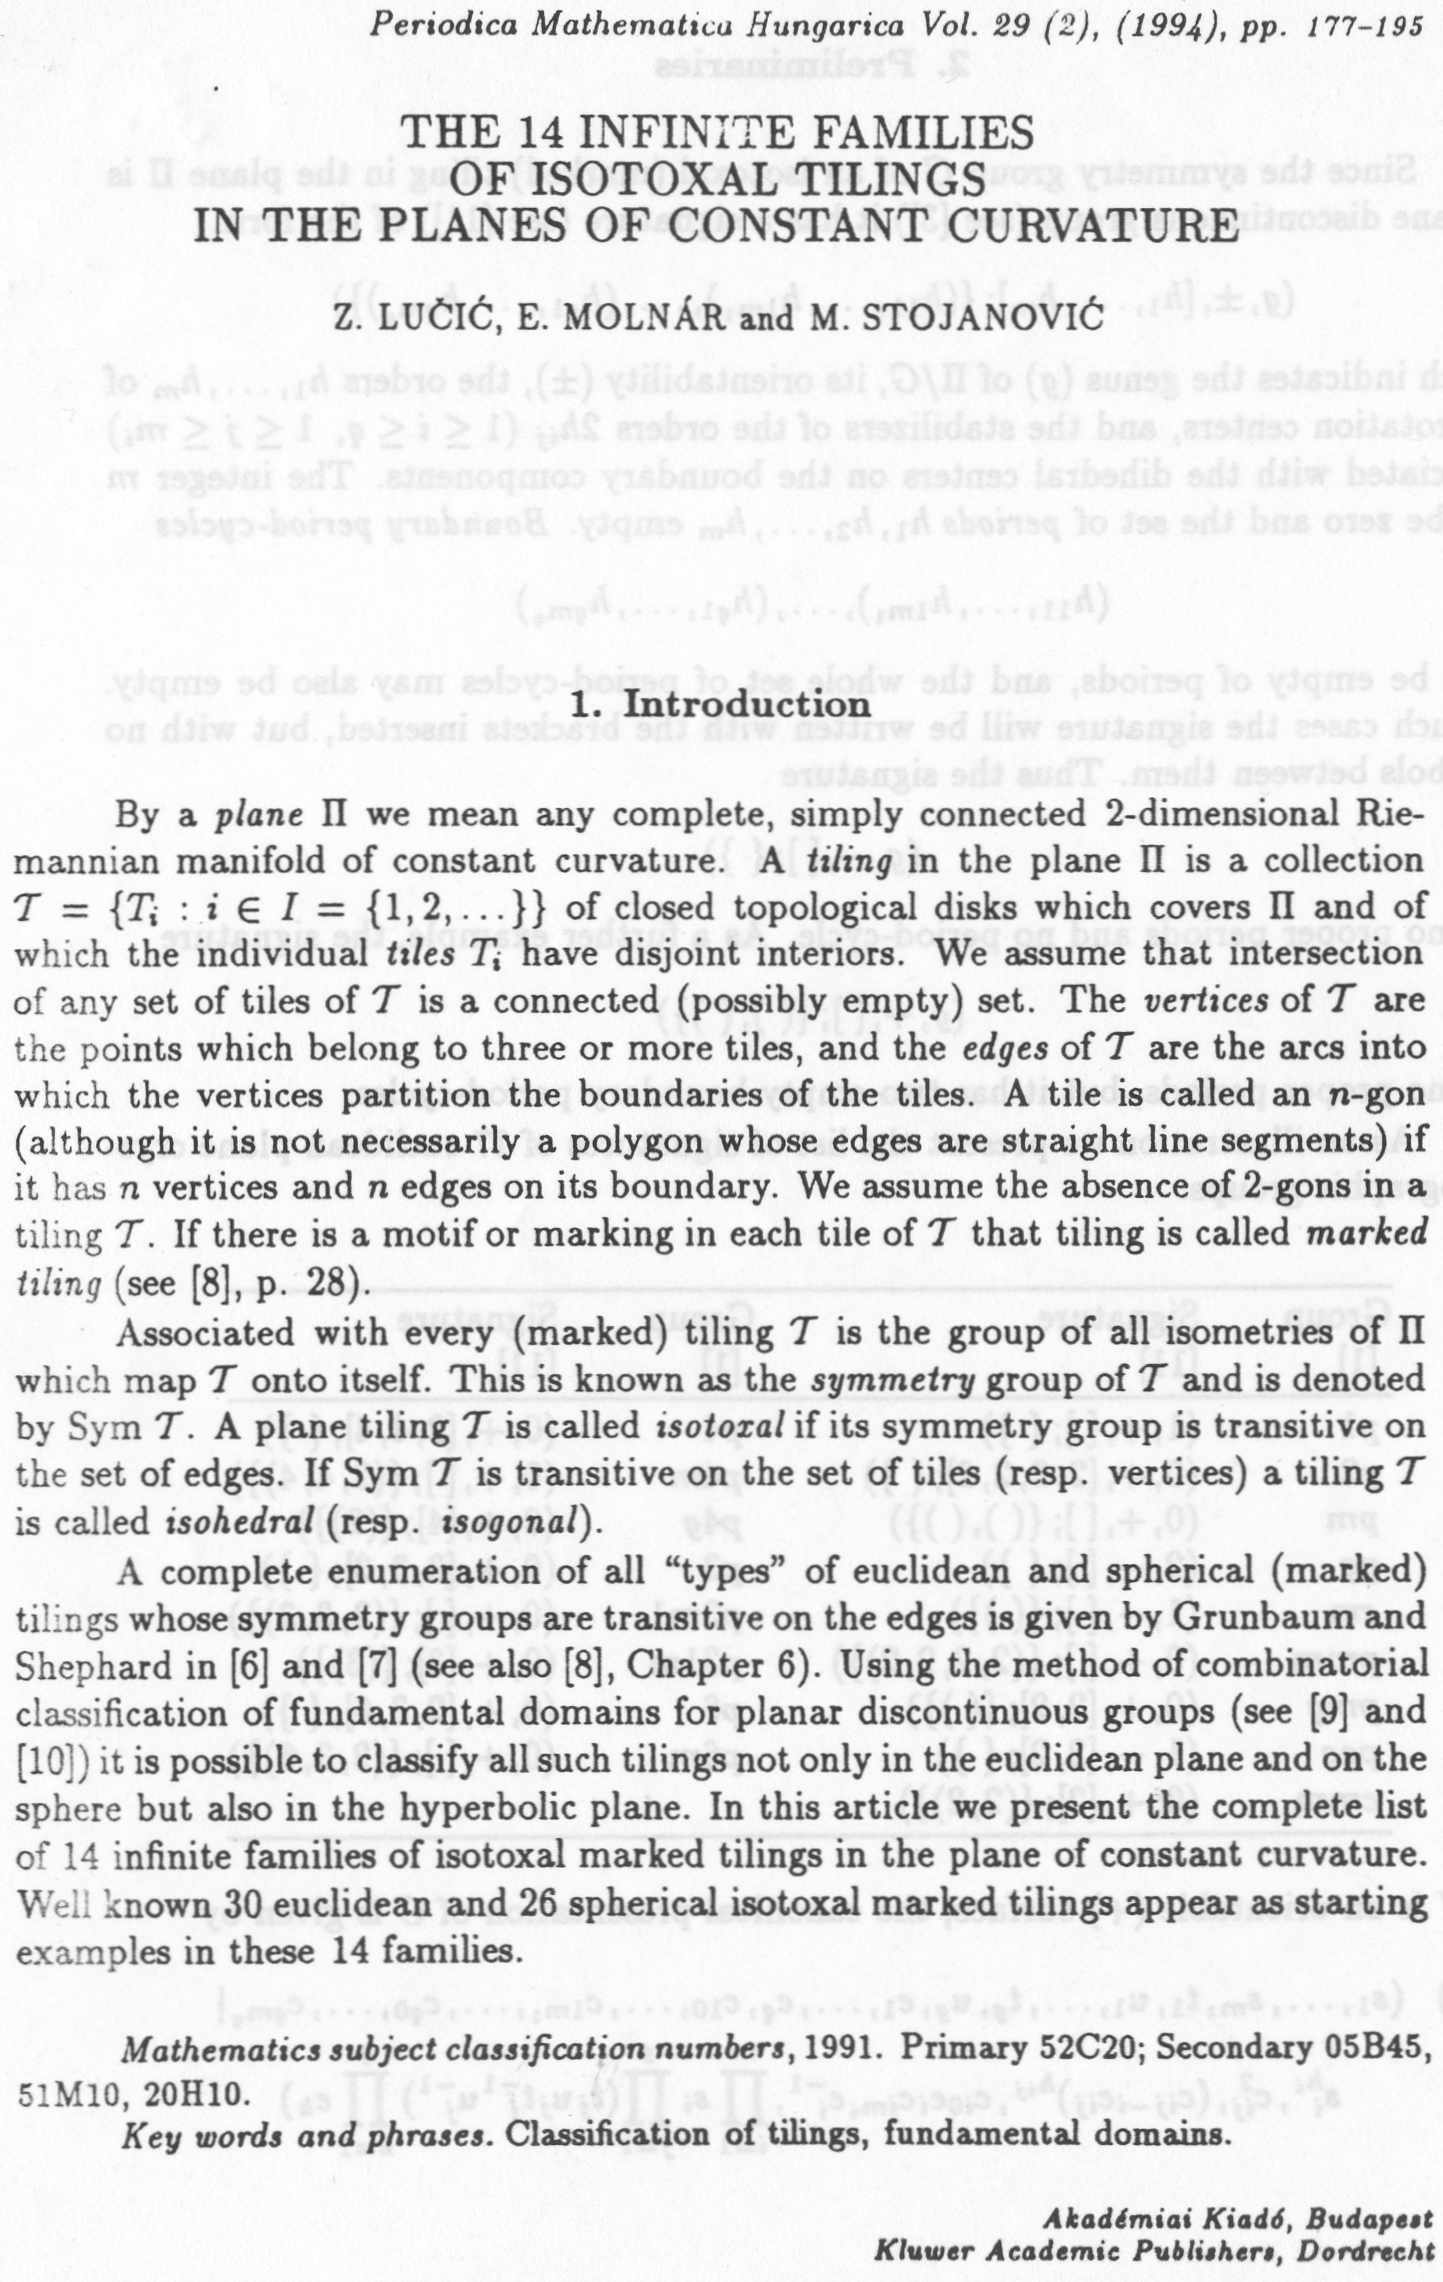
\includegraphics[width=0.6\textwidth]{illustration2.png}
\end{frame}

\section{Illustrations}
\begin{frame}
  Illustrations with square tiling in plane and with cube tilings in space.

  \center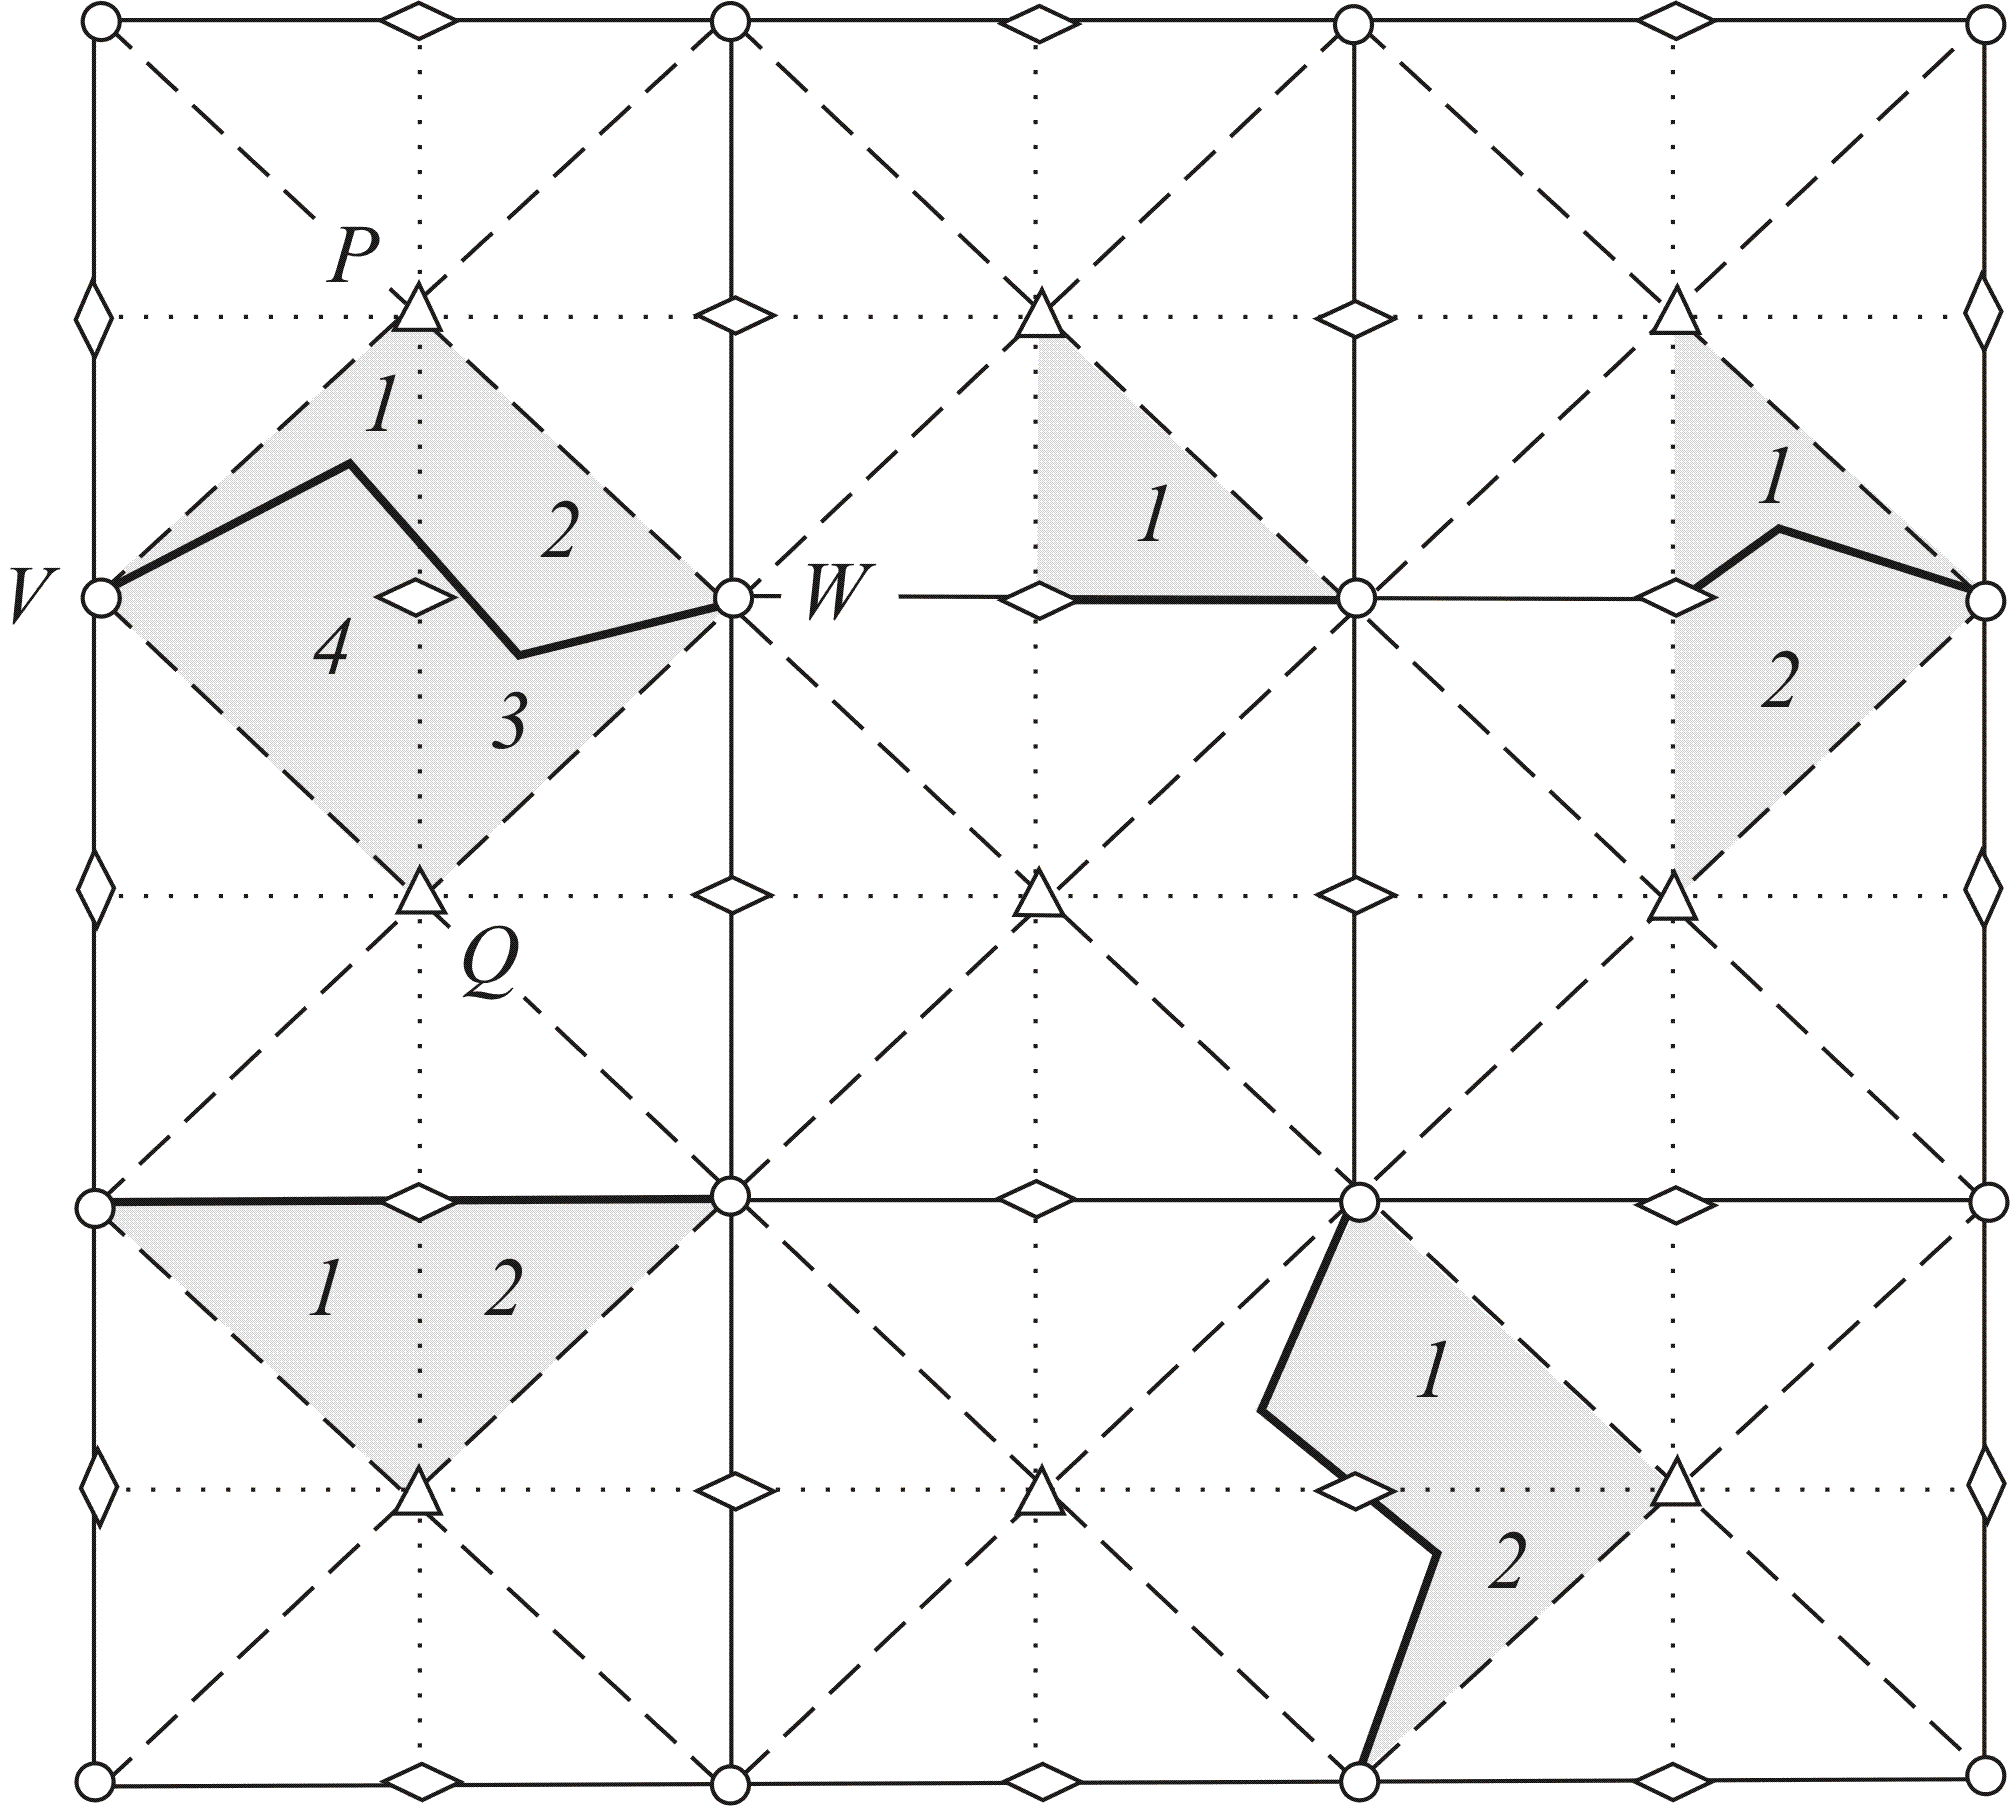
\includegraphics[width=0.7\textwidth]{illustration3.png}
\end{frame}

\begin{frame}
  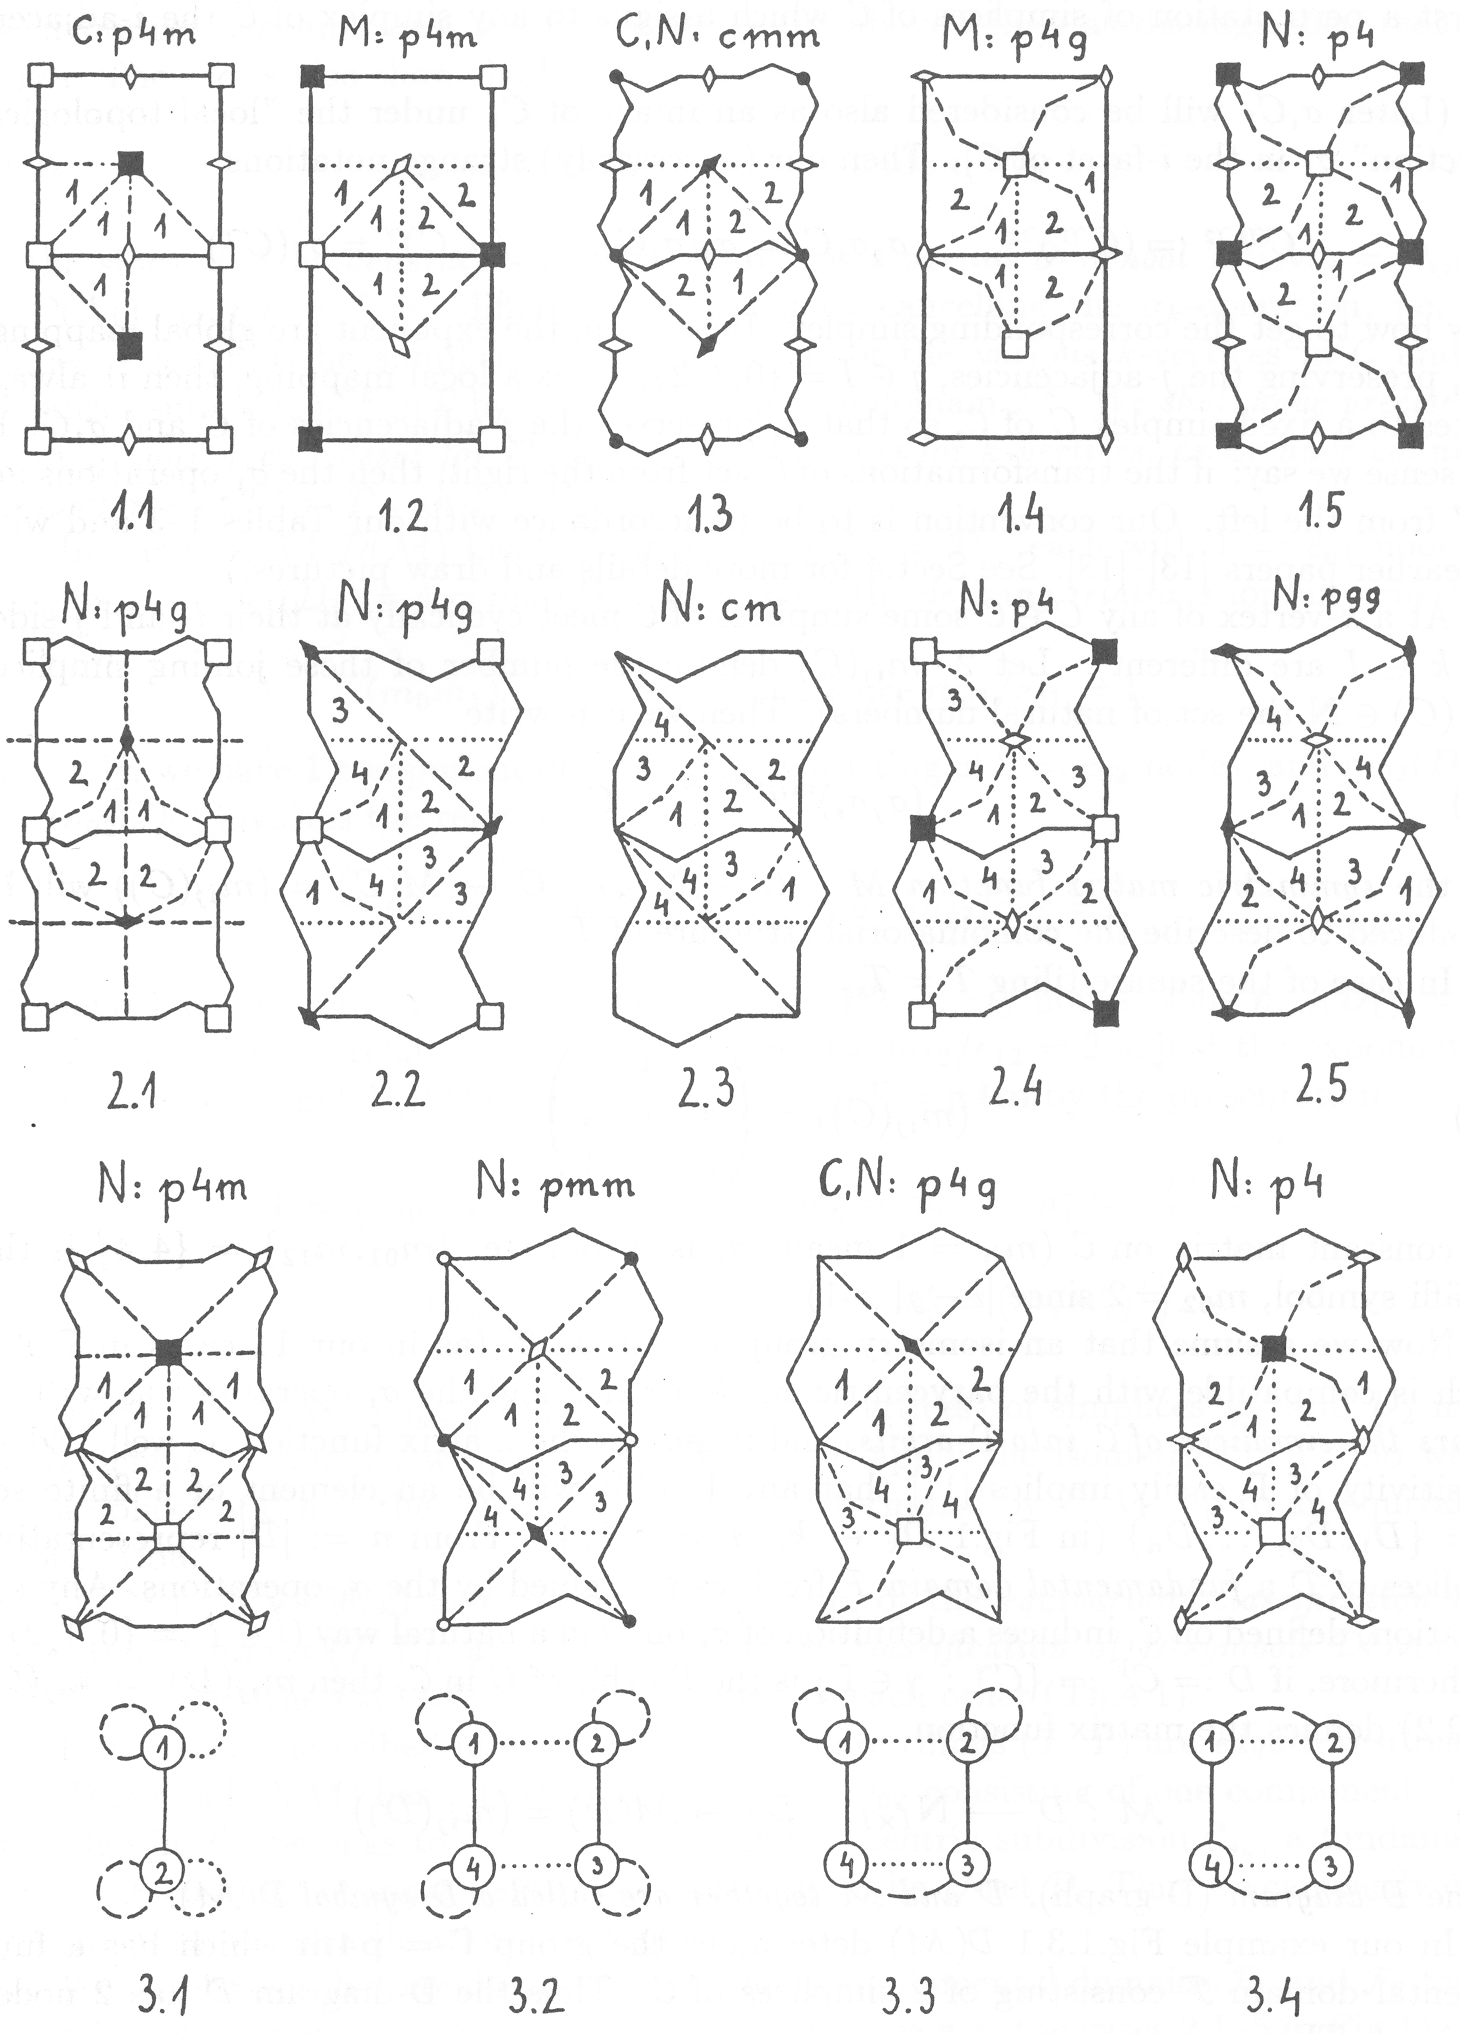
\includegraphics[width=0.7\textwidth]{illustration4.png}
\end{frame}

\begin{frame}
  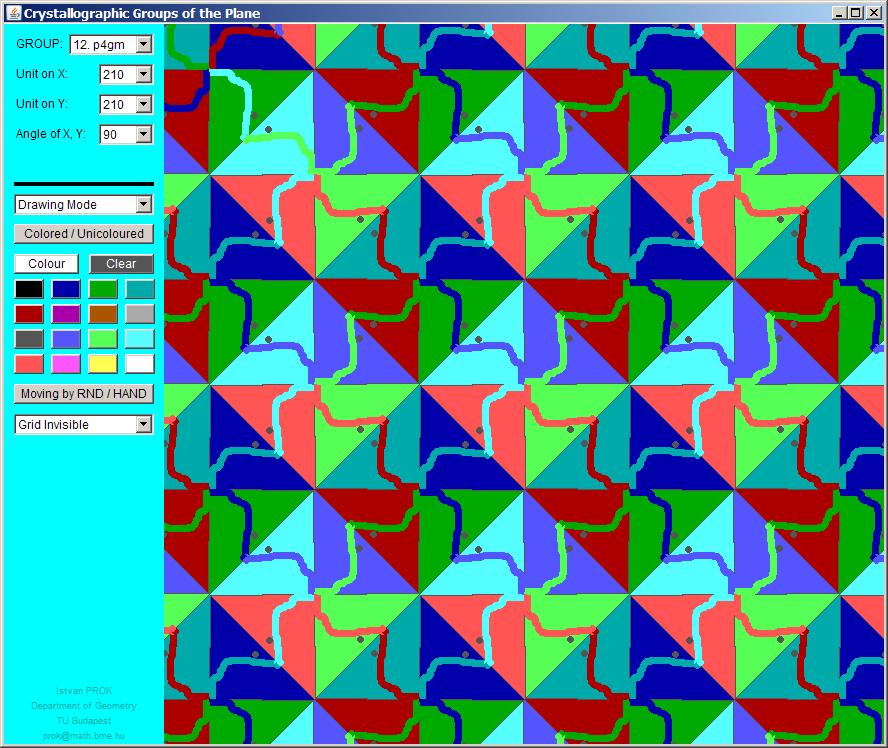
\includegraphics[width=0.9\textwidth]{illustration5.png}
\end{frame}

\begin{frame}
  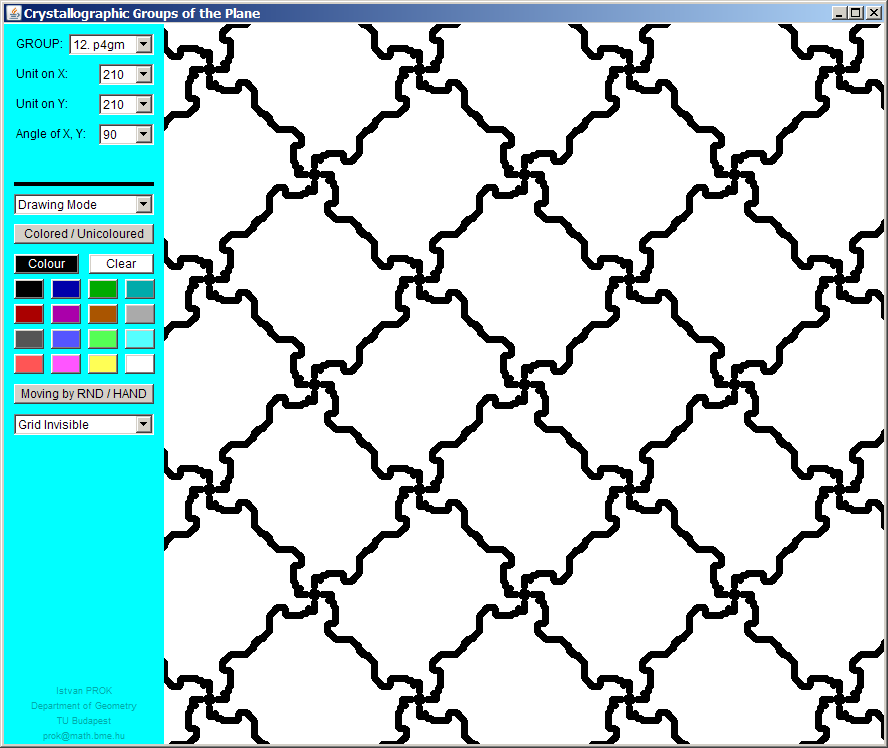
\includegraphics[width=0.9\textwidth]{illustration6.png}
\end{frame}

\begin{frame}
  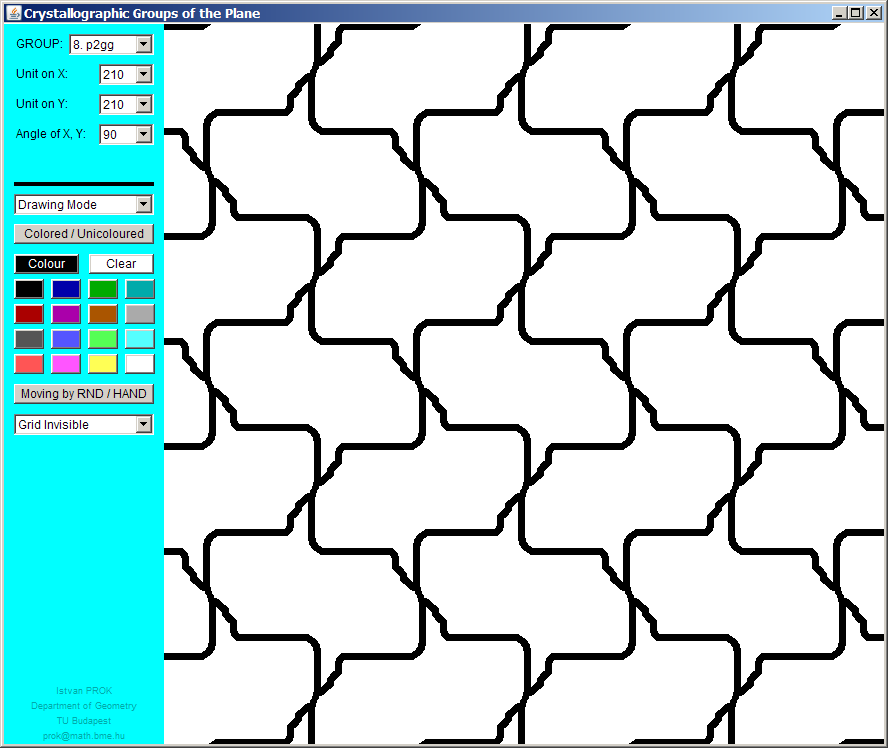
\includegraphics[width=0.9\textwidth]{illustration7.png}
\end{frame}

\begin{frame}
  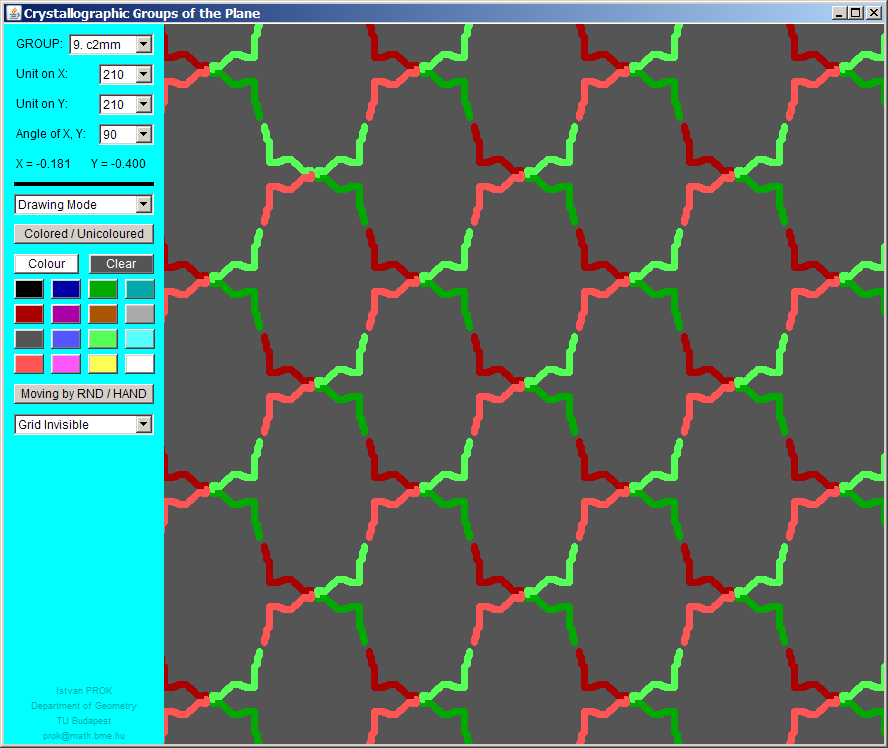
\includegraphics[width=0.9\textwidth]{illustration8.png}
\end{frame}

\section{D-symbols}
\begin{frame}
  D-symbols:
  \begin{itemize}
    \item Based on the baricentric subdivision of a tiling
    \item Structure:
      \begin{itemize}
	\item D-diagram: $dim+1$ colored graph, which represents adjacencies of
	  simplex-orbits
	\item Matrix function on simplex orbits, which represents the number of
	  simpleces (not orbits) around a $dim-2$ dimensional edge.
      \end{itemize}
    \item Constraints:
      \begin{itemize}
	\item Compatibility between the diagram and the matrix function.
	\item Compatibility with baricentric subdivision
      \end{itemize}
  \end{itemize}
\end{frame}

\section{Finding D-diagrams}
\begin{frame}
  Simple algorithm for finding D-diagrams:
  \begin{itemize}
    \item Fixed dimension and cardinality
    \item Take a fixed number of graph vertices and $dim+1$ number of colors
    \item Enumerate every possible edge-combinations and drop the "bad" and
      duplicate combinations.
    \item The algorithm can find the possible edge-transitive diagrams with a
      little perturbation.
    \item Constraints:
      \begin{itemize}
	\item Rank of vertices
	\item Patterns which makes the diagram incompatible with baricentric
	  subdivision
	\item Is the diagram connected?
	\item Permutation of vertices (ordering of diagrams)
      \end{itemize}
  \end{itemize}
\end{frame}

\section{Finding matrix-functions}
\begin{frame}
  Algorithm for finding possible matrix-functions of a D-diagram in
  $3$-dimensions:
  \begin{itemize}
    \item Parametric matrix function, minimal values
    \item $2$-dimensional subsymbols of 3 colors (simplex point stabilizers):
      \begin{itemize}
	\item Based on combinatorial curvature (decreases if we increase the
	  parameter values)
	  \begin{align*}
	    K(\leftexp{c}{\mathcal{D}}^i)=\sum_{D\in
	    \leftexp{c}{\mathcal{D}}^i}\left(-1+\sum_{\substack{0\le j<k\le 3 \\
	    j,k\ne i}}\frac{1}{m_{jk}(D)}\right)
	    \begin{array}{cccc}
	      > & & S^2 \\
	      = & 0 & \mathbb{E}^2 \\
	      < & & H^2
	    \end{array}
	  \end{align*}
	\item Only spherical or euclidean
	\item If spherical we have to exclude bad orbifolds
      \end{itemize}
    \item Increase every parameter one by one and manage infinite series
  \end{itemize}
  Some easy to answer questions:
  \begin{itemize}
    \item Does the D-symbol have proper inner symmetry (diagram and matrix function)?
    \item Does the tiling have ideal point for a given D-symbol?
  \end{itemize}
\end{frame}

\section{Example}
\begin{frame}
  Degenerate tilings:
  
  \tiny
  either $o^+=2^+$ or $p=2$ or $q=1$
  
  \begin{tabular}{|cccccccccc|}
    \hline
    & & & & & $o*q$ & $*npq2$ & $o^+*2mn$ & & \\
    $m$ & $n$ & $o^+$ & $p$ & $q=r$ & inf & inf & inf & symm & space \\
    \hline
    $1$ & $1$ & $2^+$ & $2$ & $1$ & - & - & - & - & $S^3$ \\
    & & & & $\geq2$ & - & - & - & - & $S^3$ \\
    \hline
    $1$ & $1$ & $2^+$ & $3$ & $2$ & - & - & - & - & $S^3$ \\
    & & & & $3$ & - & - & - & - & $S^3$ \\
    & & & & $4$ & - & - & - & - & $S^3$ \\
    & & & & $5$ & - & - & - & - & $H^3$ \\
    & & & & $6$ & - & + & - & - & $H^3$ \\
    \hline
    $1$ & $1$ & $2^+$ & $4$ & $2$ & - & - & - & - & $S^3$ \\
    & & & & $3$ & - & - & - & - & $E^3$ \\
    & & & & $4$ & - & + & - & - & $H^3$ \\
    & & & $5$ & $2$ & - & - & - & - & $S^3$ \\
    & & & & $3$ & - & - & - & - & $H^3$ \\
    & & & $6$ & $2$ & - & - & - & - & $S^3$ \\
    & & & & $3$ & - & + & - & - & $H^3$ \\
    \hline
    $1$ & $1$ & $2^+$ & $\geq7$ & $2$ & - & - & - & - & $S^3$ \\
    \hline
    & & $3^+$ & $2$ & $1$ & - & - & - & + & $S^3$ \\
    & & & & $2$ & - & - & - & - & $E^3$ \\
    & & & & $3$ & + & - & - & - & $H^3$ \\
    & & $4^+$ & $2$ & $1$ & - & - & + & - & $E^3$ \\
    & & & & $2$ & + & - & + & - & $H^3$ \\
    \hline
    $1$ & $2$ & $2^+$ & $2$ & $1$ & - & - & + & - & $E^3$ \\
    & & & & $2$ & - & + & + & - & $H^3$ \\
    & & & $\geq3$ & $1$ & - & - & - & - & $H^2\times R$ \\
    \hline
    $2$ & $1$ & $2^+$ & $2$ & $1$ & - & - & + & - & $E^3$ \\
    & & & & $\geq2$ & - & - & + & - & $H^2\times R$ \\
    & & & $\geq3$ & $2$ & - & - & + & - & $H^3$ \\
    \hline
  \end{tabular}
\end{frame}
\begin{frame}
  Non-degenerate tilings

  \tiny
  $o\geq3$, $p\geq3$, $q\geq2$ and $r\geq2$

  \begin{tabular}{|cccccccccc|}
    \hline
    & & & & & $o*q$ & $*npq2$ & $o^+*2mn$ & & \\
    $m$ & $n$ & $o^+$ & $p$ & $q=r$ & inf & inf & inf & symm & space \\
    \hline
    $1$ & $1$ & $3^+$ & $3$ & $2$ & - & - & - & - & $H^3$ \\
    & & & & $3$ & + & - & - & - & $H^3$ \\
    & & & $4$ & $2$ & - & - & - & + & $H^3$ \\
    & & & & $3$ & + & - & - & - & $H^3$ \\
    & & & $5$ & $2$ & - & - & - & - & $H^3$ \\
    & & & & $3$ & + & - & - & - & $H^3$ \\
    & & & $6$ & $2$ & - & - & - & - & $H^3$ \\
    & & & & $3$ & + & + & - & + & $H^3$ \\
    & & & $\geq7$ & $2$ & - & - & - & - & $H^3$ \\
    \hline
    $1$ & $1$ & $4^+$ & $\geq3$ & $2$ & + & - & + & - & $H^3$ ?! \\
    \hline
  \end{tabular}
\end{frame}
\end{document}
